\documentclass{jsarticle}
\usepackage[margin = .7in]{geometry}
\usepackage[dvipdfmx]{graphicx}
\usepackage{listings}
\usepackage{amsmath}
\usepackage{bm}
\usepackage{ascmac}
\lstset{%
  language={python},
  basicstyle={\small},%
  identifierstyle={\small},%
  commentstyle={\small\itshape},%
  keywordstyle={\small\bfseries},%
  ndkeywordstyle={\small},%
  stringstyle={\small\ttfamily},
  frame={tb},
  breaklines=true,
  columns=[l]{fullflexible},%
  numbers=left,%
  xrightmargin=0zw,%
  xleftmargin=3zw,%
  numberstyle={\scriptsize},%
  stepnumber=1,
  numbersep=1zw,%
  lineskip=-0.5ex%
}

\begin{document}
\title{卒論テーマ候補 :ゆびすま2}
\author{池上 慧}
\maketitle

\section{ゲームの概要}
\subsection{ゆびすまとは}
「ゆびすま」とは2人以上で行われるゲームである。ここでは2人で行われるケースを想定する。プレイヤーは「攻め」と「守り」の役目を交互に行う。プレイヤーは毎回好きな本数の親指を上げる。「攻め」のプレイヤーは今回上がる親指の本数を予想し、その予想した数をコールしながら、自分でも好きな本数だけ親指を上げる。「守り」のプレイヤーも掛け声と同時に親指を好きな本数だけあげる。「攻め」がコールした数と実際にあげられた親指の総数が等しかったなら「攻め」の勝ちであり、そうでなければ「引き分け」である。引き分けたら役割を交代してどちらかが勝つまで続けるものとする。本来であれば勝てば腕を一本減らすことができ、先に二回勝利した方の勝ちというルールであるが、ここでは最初の2本vs2本の状況のみを想定する。

\subsection{ゲームの構造}
このゲームで勝敗を決するのは攻め手が決定する「宣言」と「指」との差である。この差で攻め手の行動を分類することができる。すなわち相手の上げる指の数が0本の時勝利する行動の組である$\left\{ (0,0), (1,1), (2,2)\right\}$をset1とし、相手の指の数が1本の時に勝利する行動の組である$\left\{ (1,0), (2,1), (3,2)\right\}$をset2、相手の指の数が2本の時に勝利する行動の組である$\left\{ (2,0), (3,1), (4,2)\right\}$をset3とする。これを用いてゲームの利得表は以下のように与えられる。
\begin{figure}[h]
    \centering
    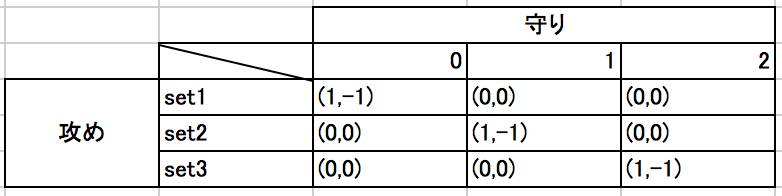
\includegraphics[width=10cm]{pmat.png}
    \caption{利得表}
\end{figure}
2人対称ゼロサムゲームとなる。守り手が$\left\{ 0,1,2\right\}$をそれぞれ取る確率を$(q,r,s)$で表記し、攻め手が取るsetに対しての混合戦略、すなわちset1, set2, set3をとる確率を$(x,y,z)$で表記する。この時の混合戦略ナッシュ均衡は以下のようである。
\begin{itembox}[l]{case1 : 完全に合理的な主体を想定したナッシュ均衡}
    \begin{align}
    	\begin{cases}
		(q, r, s) = (\frac{1}{3}, \frac{1}{3}, \frac{1}{3})\\
		(x, y, z) = (\frac{1}{3}, \frac{1}{3}, \frac{1}{3})
	\end{cases}
    \end{align}
\end{itembox}

つまり攻め手も守り手も自身の行動に等しく確率を割り振るのが最適反応を構成している。この時攻め手の本来の行動である$9$個の「宣言」と「指」のペアに対しても等しく$\frac{1}{9}$ずつ確率が振られている。

\section{研究の目的意識}
しかし上記のように全ての戦略に等しく確率を割り振る戦略が実際のプレイでは取られていない可能性が高い。$[a,b]$で宣言$a$ゆびの数$b$の攻め手の行動を表すことにすると、経験的には$[2,1]$のようなある種中途半端な戦略が$[0,0]$や$[4,2]$のような極端な戦略よりも取られやすい傾向があるようように思える。実際、地域によっては利得構造は変えずに$[0,0]$と$[4,2]$に対して特別な名称を与え、他の行動とは別物として扱われているようである。

限定合理性のモデル化によって上記の現象が説明できないかを考える。2人完備情報ゲームに適用可能な限定合理生のモデルとして代表的なものにはOsborn and Rubinshtein (1998)で提案されたS(k) EquilibriumやMcKelvey and Palfrey (1995)で提案されたquantal response equilibriumなどがある。しかし、先に挙げたこのゲームの利得表を見ればわかる通りゆびすまは対称なゲームである。このような単純な構造を持つゲームにおいて特定の行動が特別選ばれがちになるような限定合理生のモデルは既存のモデルには見当たらず、実際上記の二つの計算結果は先のナッシュ均衡と同じになってしまう。

ここではこの現象を説明する方向性として、ゲームの基幹とも言える行動主体とその取りうる行動に関する認識自体が完全ではない時にどのような行動がとられるかを分析する。具体的には以下の二つの軸でゲームの構造への誤認が発生している状況を考える。
\begin{enumerate}
	\item 相手主体を分割し異なる複数主体が相手の手を構成しているかのように誤認する(擬人化)
	\item 複数要素の組み合わせで表現される自身の行動を組み合わせそのものとして捉えることができず個別要素ごとに最適行動を取ろうとする(統合失敗)
\end{enumerate}

ゆびすまにおいて具体的に見ていく。本来は$\left\{ 0,1,2 \right\}$である守り手の行動について誤認が発生するのが一つ目の非合理性であり、そこでは相手のゆびがそれぞれ別の主体によって動かされているという想定の下行動することになる。すなわち本来2人ゲームであるゆびすまを3人ゲームであるかのように振舞うことになる。ゆびすまにおいてこのような誤認が発生しうるであろう根拠としてはゲームの進行にしたがって指が1本ずつ減らされていくという点が挙げられる。今回の研究ではこの2本vs2本の状況しか扱わないが、ゆびすまは広く知られたゲームであるためこの認識はどのプレイヤーにも浸透していると考えられる。

一方で、攻め手が「宣言」と「指」の組み合わせとして自身の行動が決まっているという認識を正しく持てない状況が二つ目の非合理性である。「宣言」を縦軸に、「指」を横軸にした表の上で攻め手の行動を考える。
\begin{figure}[h]
    \centering
    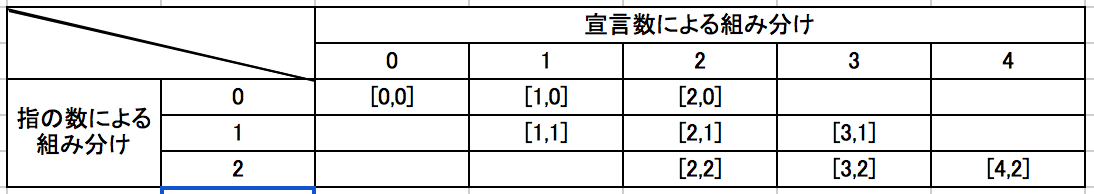
\includegraphics[width=10cm]{class2.png}
    \caption{組み分け}
\end{figure}
まず、自身の行動を組み合わせとして正しく認識しているということが何を指すのかを考える。組み合わせとして正しく認識しているとは、図1のような利得表がこのゲームの利得表であるということを正しく認識した上でゲームをプレイするということである。すなわちさきに述べたset1からset3がそれぞれ同じ勝利条件であることを認識し、setごとに混合戦略の確率を振ることができる状況である。図2の表でいうと、$9$個の組み合わせに対して斜めに3つずつのグループ分けをしている状況である。


\end{document}



































